%%% File: ./inputs/parts/DIGITAL_ASSISTANTS.tex

%%% %%%%%%%%%%%%%%%%%%%%%%%%%%%%%%%%%%%%%%%%%%%%%%%%%%%%%%%%%%%%%%%%%%%%%%%%%%%%

%%% \begin{quotation}
%%% %
%%%   We focus on automated programming for several reasons: deep neural networks have recently demonstrated progress on automated code synthesis and program repair by leveraging existing technologies; computers and, in particular, modern integrated development environments present a rich alternative to the dominant simulation environments; programming is challenging for humans and machines alike and we foresee opportunities to increase the productivity of software engineers. That said, in this section we emphasize basic tools that enable the assistant to encode, represent and manipulate fully differentiable programs.
%%% % 
%%% \end{quotation}

We focus on automated programming for several reasons: deep neural networks have recently demonstrated progress on automated code synthesis and program repair by leveraging existing technologies; computers and, in particular, modern integrated development environments present a rich alternative to the dominant simulation environments; programming is challenging for humans and machines alike and we foresee opportunities to increase the productivity of software engineers. That said, in this section we emphasize basic tools that enable the assistant to encode, represent and manipulate fully differentiable programs.

%%% %%%%%%%%%%%%%%%%%%%%%%%%%%%%%%%%%%%%%%%%%%%%%%%%%%%%%%%%%%%%%%%%%%%%%%%%%%%%

%%%%%%%%%%%%%%%%%%%%%%%%%%%%%% BEGIN PROCEDURAL MODEL %%%%%%%%%%%%%%%%%%%%%%%%%%

The integrated development environment and its associated software engineering tools constitute an extension of the apprentice’s capabilities in much the same way that a piano or violin extends a musician or a prosthetic limb extends someone who has lost an arm or leg. The extension becomes an integral part of the person possessing it and over time their brain creates a topographic map that facilitates interacting with the extension\footnote{%
%
  In the mammalian brain, information pertaining to sensing and motor control is topographically mapped to reflect the intrinsic structure of that information required for interpretation. This was early recognized in the work of Hubel and Wiesel~\cite{HubelandWieselJoP-68,HubelandWieselJoP-62} on the striate cortex of the cat and macaque monkey and in the work of Wilder Penfield~\cite{PenfieldandBoldreyBRAIN-37} developing the idea of a cortical homunculus in the primary motor and somatosensory areas of the brain located between the parietal and frontal lobes of the primate cortex. Such maps have become associated with the theory of embodied cognition.}. 
 
As engineers designing the apprentice, part of our job is to create tools that enable the apprentice to learn its trade and eventually become an expert. Conventional IDE tools simplify the job of software engineers in designing software. The fully instrumented IDE (FIDE) that we engineer for the apprentice will be integrated into the apprentice’s cognitive architecture so that tasks like stepping a debugger or setting breakpoints are as easy for the apprentice as balancing parentheses and checking for spelling errors in a text editor is for us.

As a first step in simplifying the use of FIDE for coding, the apprentice is designed to manipulate programs as abstract syntax trees (AST) and easily move back and forth between the AST representation and the original source code in collaborating with the programmer. Both the apprentice and the programmer can modify or make references to text appearing in the FIDE window by pointing to items or highlighting regions of the source code. The text and AST versions of the programs represented in the FIDE are automatically synchronized so that the program under development is forced to adhere to certain syntactic invariants. 

%%% %%%%%%%%%%%%%%%%%%%%%%%%%%%%%%%%%%%%%%%%%%%%%%%%%%%%%%%%%%%%%%%%%%%%%%%%%%%%

%%% Figure~{\urlh{#fig_Differentiable_Structured_Programs}{\ref{fig_programs}}}
\begin{figure}
%
  \begin{center} 
%    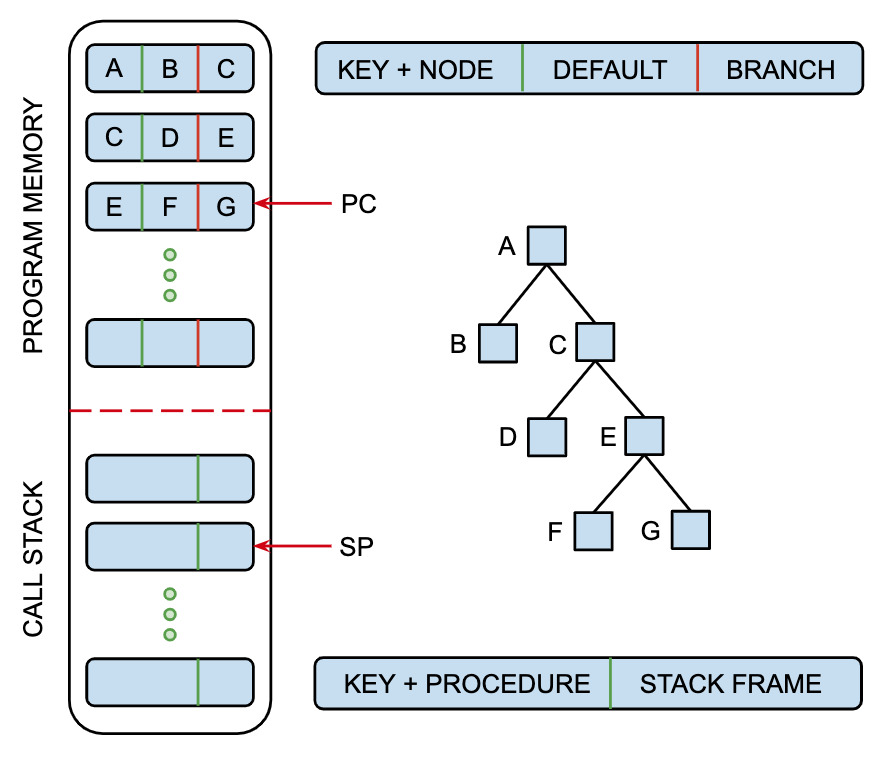
\includegraphics[width=5.9375in]{./figures/Differentiable_Structured_Programs.png} % 625 × 528 pixels
    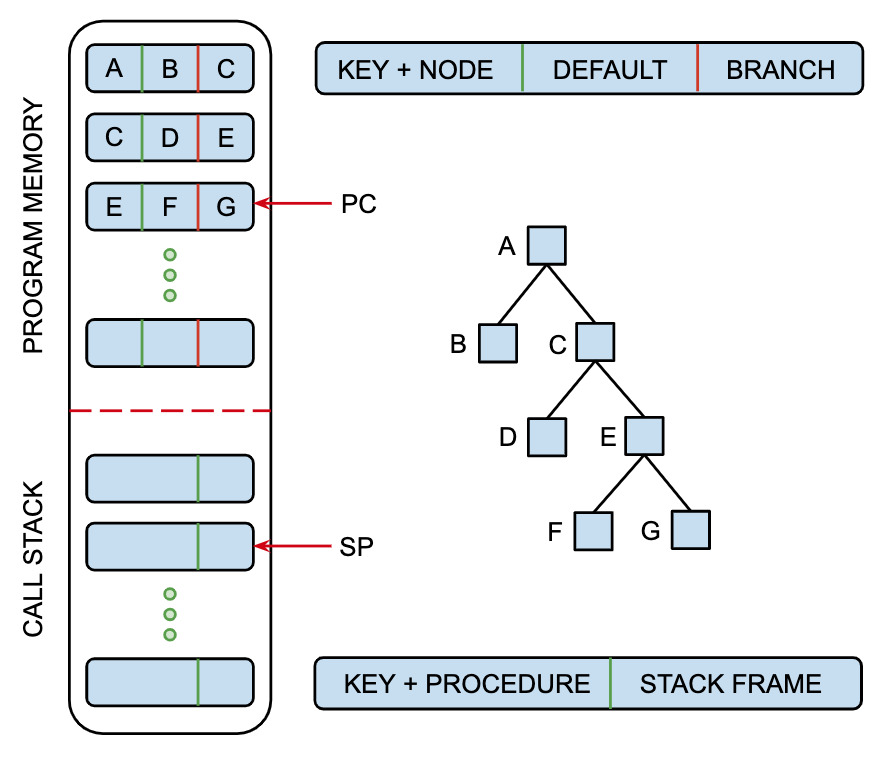
\includegraphics[width=3in]{./figures/Differentiable_Structured_Programs.png} % 625 × 528 pixels
  \end{center}
%
  \caption{We use pointers to represent programs as abstract syntax trees and partition the NTM memory, as in a conventional computer, into program memory and a LIFO execution (call) stack to support recursion and reentrant procedure invocations, including call frames for return addresses, local variable values and related parameters. The NTM controller manages the program counter and LIFO call stack to simulate the execution of programs stored in program memory. Program statements are represented as embedding vectors and the system learns to evaluate these representations in order to generate intermediate results that are also embeddings. It is a simple matter to execute the corresponding code in the FIDE and incorporate any of the results as features in embeddings.}
%
  \label{fig_programs}
%
\end{figure}

%%% %%%%%%%%%%%%%%%%%%%%%%%%%%%%%%%%%%%%%%%%%%%%%%%%%%%%%%%%%%%%%%%%%%%%%%%%%%%%

To support this hypothesis, we are developing distributed representations for programs that enable the apprentice to efficiently search for solutions to programming problems by allowing the apprentice to easily move back and forth between the two paradigms, exploiting both conventional approaches to program synthesis and recent work on machine learning and inference in artificial neural networks. Neural Turing Machines coupled with reinforcement learning are capable of learning simple programs~\cite{GravesetalCoRR-14}. We are interested in representing structured programs expressed in modern programming languages. Our approach is to alter the NTM controller and impose additional structure on the NTM memory designed to support procedural abstraction. 

%%%%%%%%%%%%%%%%%%%%%%%%%%%%%% END PROCEDURAL MODEL %%%%%%%%%%%%%%%%%%%%%%%%%%%%

%%%%%%%%%%%%%%%%%%%%%%%%%%%%%% BEGIN EXECUTION_MODEL.tex %%%%%%%%%%%%%%%%%%%%%%%

What could we do with such a representation? It is important to understand why we don’t work with some intermediate representation like bytecodes. By working in the target programming language, we can take advantage of both the abstractions afforded by the language and the expert knowledge of the programmer about how to exploit those abstractions. The apprentice is bootstrapped with several statistical language models: one trained on a natural language corpus and the other on a large code repository. Using these resources and the means of representing and manipulating program embeddings, we intend to train the apprentice to predict the next expression in a partially constructed program by using a variant of imagination-based planning~\cite{PascanuetalCoRR-17}. As another example, we will attempt to leverage NLP methods to generate proposals for substituting one program fragment for another as the basis for code completion. 

%%% %%%%%%%%%%%%%%%%%%%%%%%%%%%%%%%%%%%%%%%%%%%%%%%%%%%%%%%%%%%%%%%%%%%%%%%%%%%%

%%% Figure~{\urlh{#fig_Differentiable_Program_Emulation}{\ref{fig_emulator}}}
\begin{figure}
%
  \begin{center} 
%    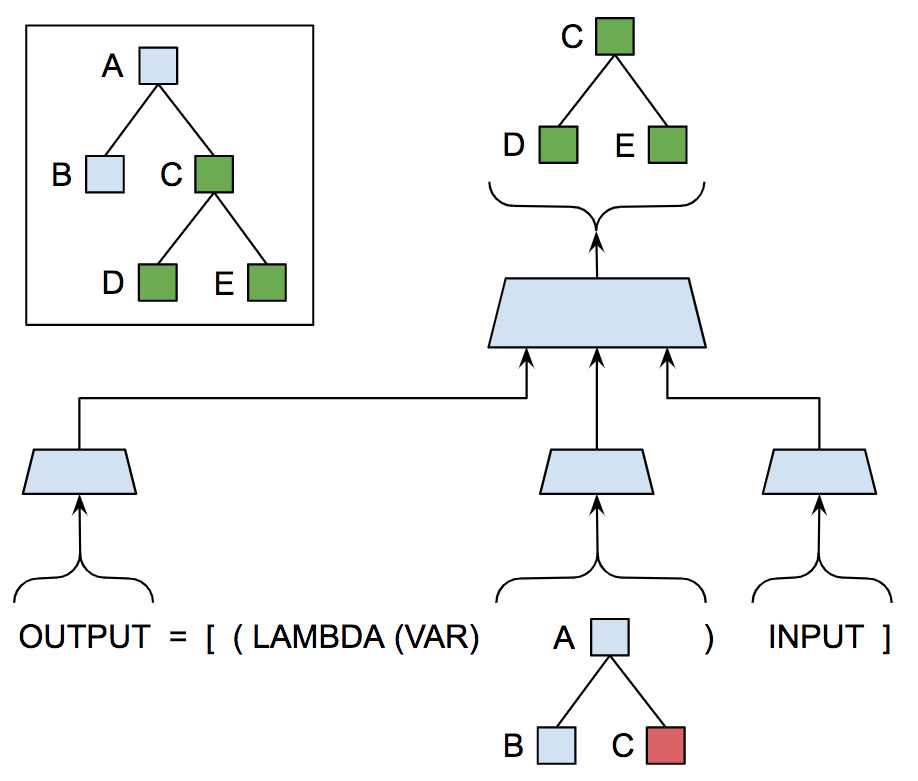
\includegraphics[width=5.3125in]{./figures/Differentiable_Program_Emulation.png} % 918 × 781 pixels
    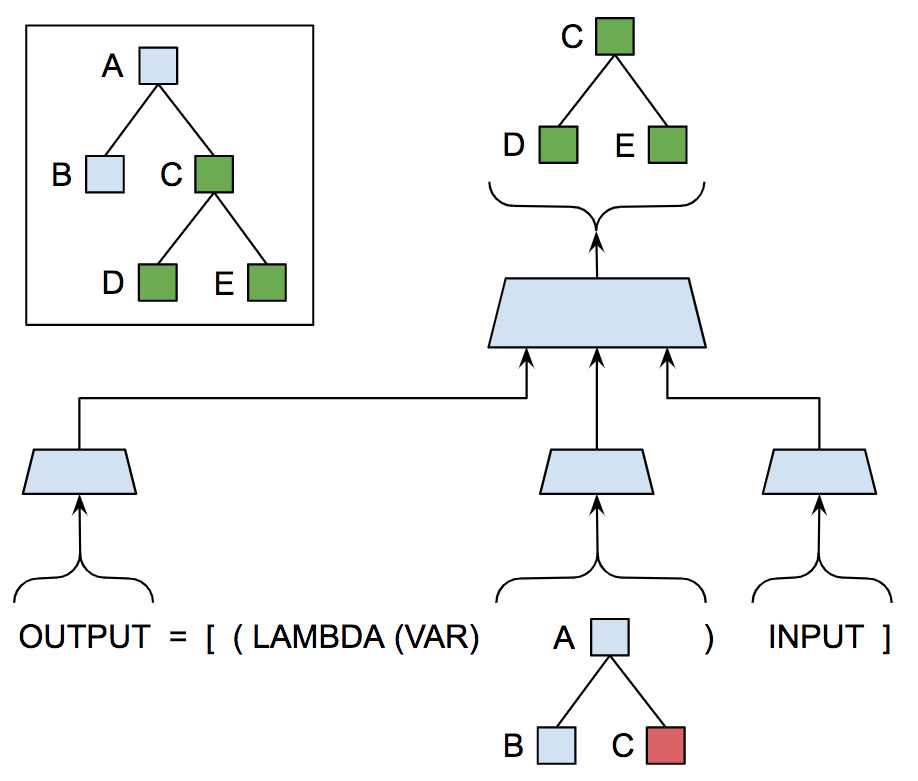
\includegraphics[width=2.65in]{./figures/Differentiable_Program_Emulation.png} % 918 × 781 pixels
  \end{center}
%
  \caption{This slide illustrates how we make use of input / output pairs as program invariants to narrow search for the next statement in the evolving target program. At any given moment the call stack contains the trace of a single conditioned path through the developing program. A single path is unlikely to provide sufficient information to account for the constraints implicit in all of the sample input / output pairs and so we intend to use a limited lookahead planning system to sample multiple execution traces in order to inform the prediction of the next program statement. 
%
These so-called imagination-augmented agents implement a novel architecture for reinforcement learning that balances exploration and exploitation using imperfect models to generate trajectories from some initial state using actions sampled from a rollout policy~\cite{PascanuetalCoRR-17,WeberetalCoRR-17,HamricketalCoRR-17,GuezetalCoRR-18}. These trajectories are then combined and fed to an output policy along with the action proposed by a model-free policy to make better decisions. There are related reinforcement learning architectures that perform Monte Carlo Markov chain search to apply and collect the constraints from multiple input / output pairs.}
%
  \label{fig_emulator}
%
\end{figure}

%%% %%%%%%%%%%%%%%%%%%%%%%%%%%%%%%%%%%%%%%%%%%%%%%%%%%%%%%%%%%%%%%%%%%%%%%%%%%%%

The Differentiable Neural Program (DNP) representation and associated NTM controller for managing the call stack and single-stepping through such programs allow us to exploit the advantages of distributed vector representations to predict the next statement in a program under construction. This model makes it easy to take advantage of supplied natural language descriptions and example input / output pairs plus incorporate semantic information in the form of execution traces generated by utilizing the FIDE to evaluate each statement and encoding information about local variables on the stack.

%%%%%%%%%%%%%%%%%%%%%%%%%%%%%% END EXECUTION_MODEL.tex  %%%%%%%%%%%%%%%%%%%%%%%%

%%%%%%%%%%%%%%%%%%%%%%%%%%%% BEGIN PROGRAMMING MODEL %%%%%%%%%%%%%%%%%%%%%%%%%%%

The imagination-based planning (IBP) for reinforcement learning framework~\cite{PascanuetalCoRR-17} serves as an example for how the code synthesis module might be implemented. The IBP architecture combines three separate adaptive components: (a) the {\it{controller}} + {\it{memory}} system which maps a state $s \in S$ and history $h \in H$ to an action $a \in A$; (b) the {\it{manager}} maps a history $h \in H$ to a route $u \in U$ that determines whether the system performs an action in the {\it{compute}} environment, e.g., single-step the program in the FIDE, or performs an imagination step, e.g., generates a proposal for modifying the existing code under construction; the {\it{imagination model}} is a form of dynamical systems model that maps a pair consisting of a state $s \in S$ and an action $a \in A$ to an imagined next state $s' \in S$ and scalar-valued reward $r \in R$.

The imagination model can be implemented as an interaction network~\cite{BattagliaetalNIPS-16} or using the graph-networks framework~\cite{BattagliaetalCoRR-18,SanchezetalCoRR-18}. The three components are trained by three distinct, concurrent, on-policy training loops. The IBP framework shown in Figure~{\urlh{#Graph_Nets_Imagination_Coding}{\ref{fig_imagine}}} allows code synthesis to alternate between exploiting by modifying and running code, and exploring by using the model to investigate and analyze what would happen if you actually did act. The manager chooses whether to execute a command or predict (imagine) its result and can generate any number of trajectories to produce a tree $h_t$ of imagined results. The controller takes this tree plus the compiled history and chooses an action (command) to carry out in the FIDE.

%%% %%%%%%%%%%%%%%%%%%%%%%%%%%%%%%%%%%%%%%%%%%%%%%%%%%%%%%%%%%%%%%%%%%%%%%%%%%%%

%%% Figure~{\urlh{#Graph_Nets_Imagination_Coding}{\ref{fig_imagine}}}
\begin{figure}
%
  \begin{center} 
%    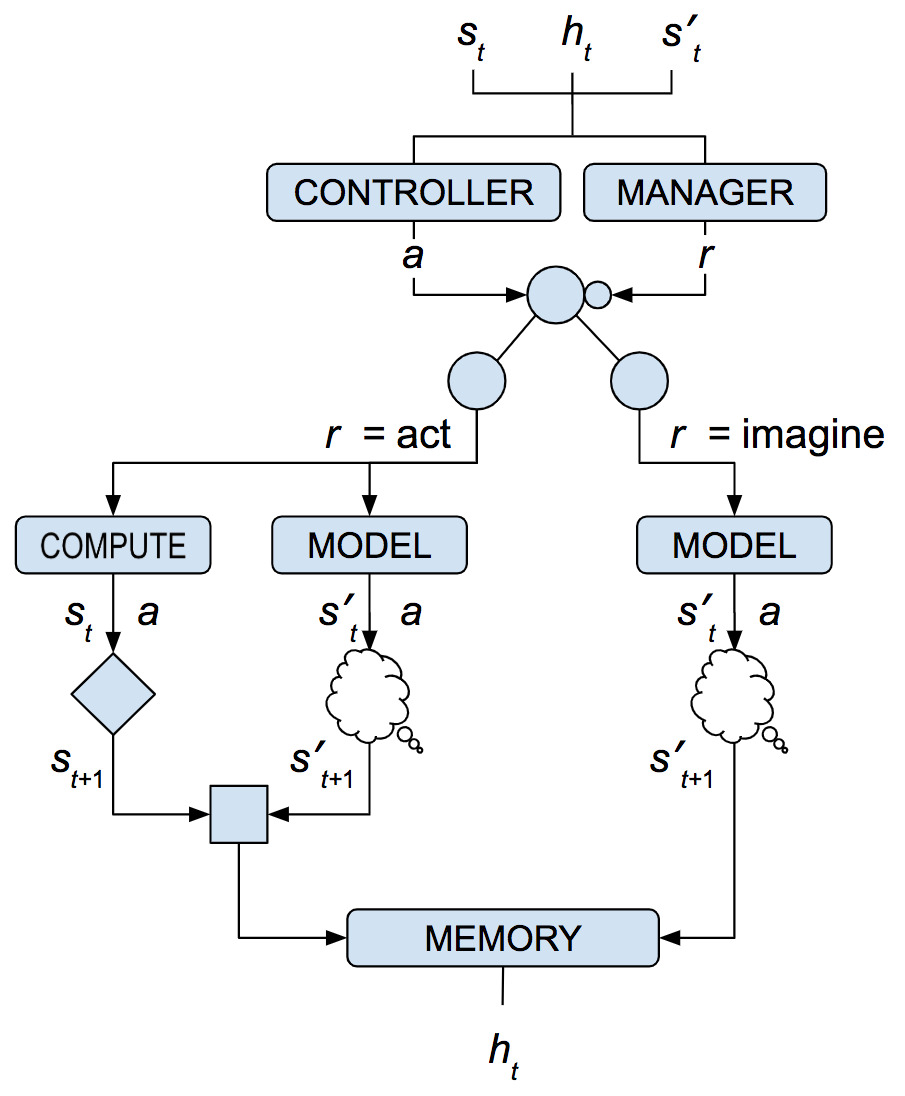
\includegraphics[width=4.3125in]{./figures/Graph_Nets_Imagination_Coding.png} % 905 × 1096 pixels
    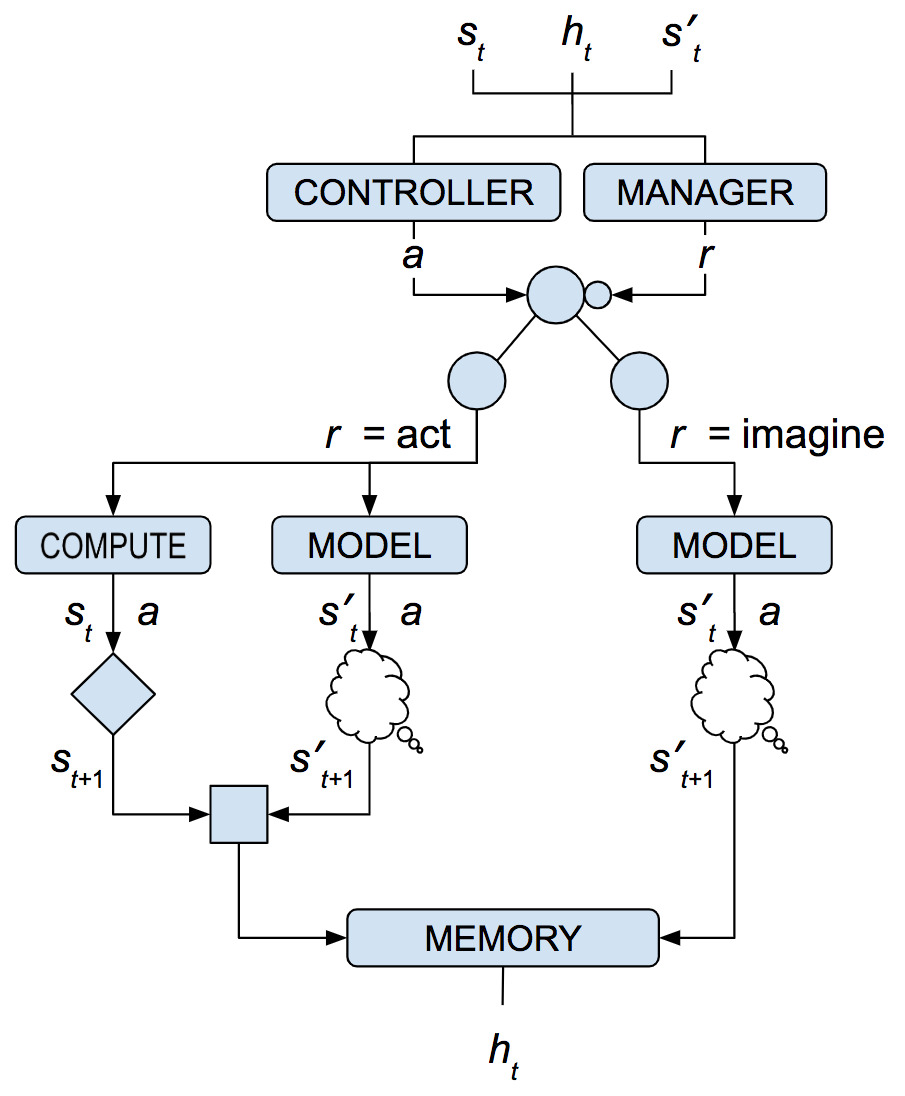
\includegraphics[width=2.15in]{./figures/Graph_Nets_Imagination_Coding.png} % 905 × 1096 pixels
  \end{center}
%
  \caption{The above graphic illustrates how we might adapt the imagination-based planning (IBP) for reinforcement learning framework~\cite{PascanuetalCoRR-17} for use as the core of the apprentice code synthesis module. Actions in this case correspond to transformations of the program under development. States incorporate the history of the evolving partial program. Imagination consists of exploring sequences of program transformations.}
%
  \label{fig_imagine}
%
\end{figure}

%%%%%%%%%%%%%%%%%%%%%%%%%%%%%% END PROGRAMMING MODEL %%%%%%%%%%%%%%%%%%%%%%%%%%%


%%% %%%%%%%%%%%%%%%%%%%%%%%%%%%%%%%%%%%%%%%%%%%%%%%%%%%%%%%%%%%%%%%%%%%%%%%%%%%%